\subsection{Histogram Computation}\label{sec:histogram}

A histogram succinctly summarizes the distribution of sample values, and thus is useful as a cursory
``look'' into the data and in guiding further analysis. For example, it can be used to guide the
selection of colors and opacities in a transfer function.

To decide on an error metric to compare histograms, we have experimented with several popular
metrics such as Kolmogorov-Smirnov \todo{cite}, Kullback-Leibler \todo{cite}, Earth Mover's
Distance~\cite{emd1998} among others (Hellinger \todo{cite}, Total variation \todo{cite}, Chi-square
\todo{cite}, Bhattacharyya \todo{cite}). We choose histogram
intersection~\cite{histogram_intersection1991} as the metric of choice, because it is fast to
compute and is reasonably insensitive to changes in precision, as well as the number of bins. The
intersection distance between two histograms $H_1$ and $H_2$ is defined as
$\err(H_1,H_2)=1-\sum_{i}{\min{(H_1(i),H_2(i))}}$ (the sum is over all bins $i$). Every histogram is
normalized by dividing the value in each bin by the number of samples in the volume. The error
metric should take into account both the histogram shapes and the range of values. Therefore, we
clamp the range of values in reconstructed fucntions to that of the original function, so that
corresponding histogram bins, i.e., $H_1(i)$ and $H_2(i)$, share the same range.

As before, for each data set, we use~\Cref{alg:greedy} to compute an \shop stream, optimized for
histogram error, and then construct an \shsg from its signature. We plot the error curves for all
relevant streams using the Intersection error metric~(compare
\Cref{fig:histogram-stream-comparison}). We use 64 for the number of bins, but note that there exist
no meaningful differences across a wide range of number of bins (from 64 to 512) in our experiments.
In all cases, the group consisting of \sbit, \slvl, and \smag underperforms the other group by a
large margin.

Among the former group of streams, \slvl generally outperforms \sbit at low bit rates, although
there are several crossover points between the two curves~(visualization
in~\Cref{fig:histogram-explain}). When leading zero packets are present, \slvl outperforms \sbit,
because increasing resolution does not help produce an accurate histogram as much as increasing
precision. The histogram is oblivious to spatial locations of samples (which require resolution to
resolve), but is sensitive to sample values (which require precision). However, when leading zero
packets are removed with compression, \sbit benefits significantly more than \slvl does (for the
same reason explained in~\Cref{sec:rmse-optimized}), resulting in the observed crossovers. Finally,
\smag performs poorly, because it ignores regions of smooth variations, which nevertheless count
toward the distribution.

In the latter group, the performances of \swav and \shsg (and even \shop) differ by negligible
amount. This observation is confirmed in~\Cref{fig:histograms-boiler}, where we plot various
histograms, reconstructed at 0.13 bps, for the \emph{boiler} data set. The histograms produced by
\swav and \shsg have approximately the same shape, and are the closest to the reference histogram.
The next best histogram is produced by \slvl, followed by the one produced by \sbit, and finally
\smag. These results suggest that histogram computation, while being in favor of precision, benefits
significantly from a bit ordering that combines both resolution and precision, not one that adheres
to either exclusively.

\begin{figure*}[t]
	\centering
	\subcaptionbox{\emph{boiler}}
	{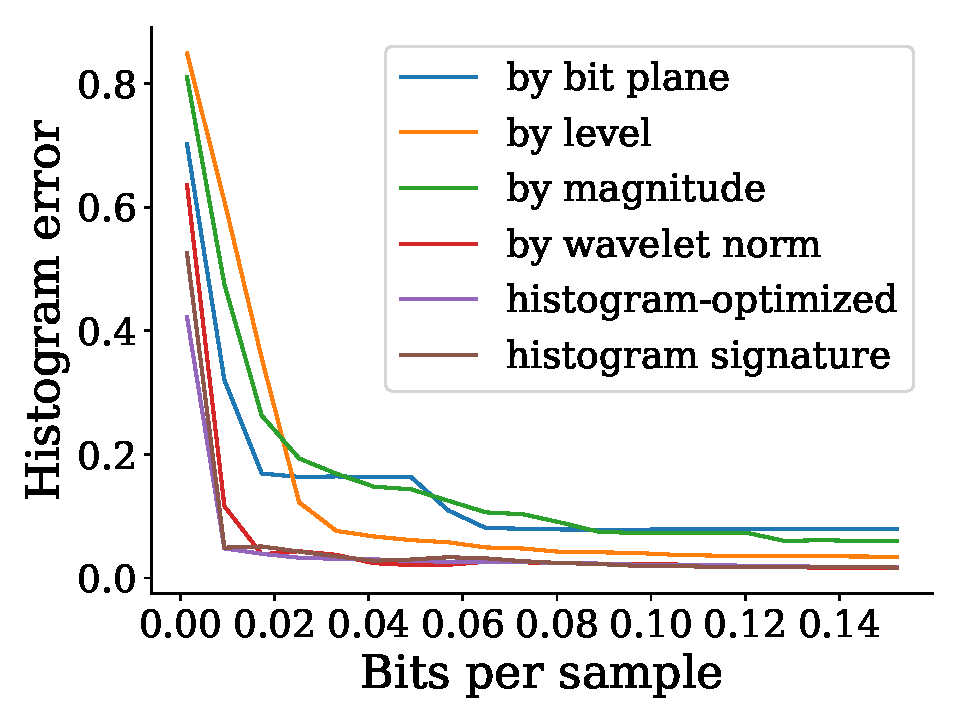
\includegraphics[width=0.24\linewidth]{histogram/histogram-optimized-boiler}}
	\subcaptionbox{\emph{diffusivity}}
	{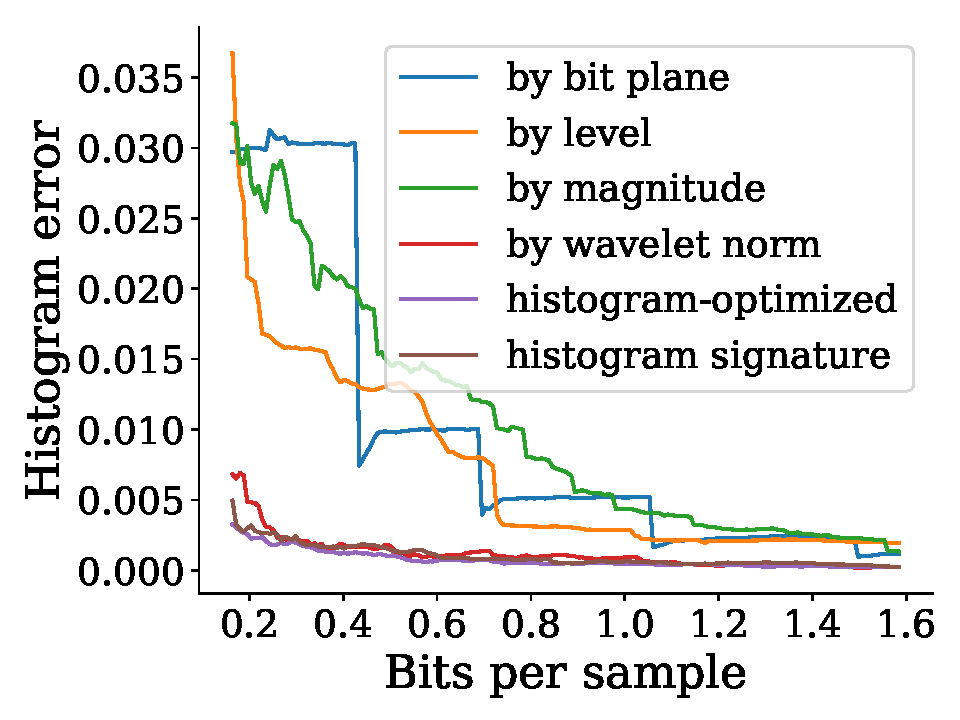
\includegraphics[width=0.24\linewidth]{histogram/histogram-optimized-diffusivity}}
	\subcaptionbox{\emph{kingsnake}}
	{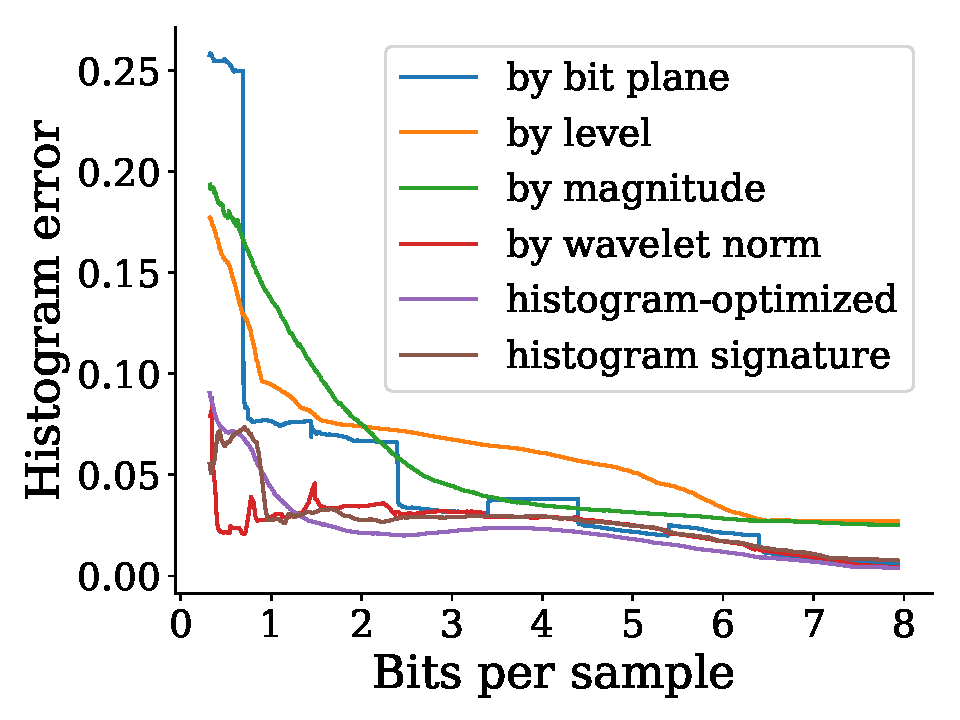
\includegraphics[width=0.24\linewidth]{histogram/histogram-optimized-kingsnake}}
	\subcaptionbox{\emph{foam}}
	{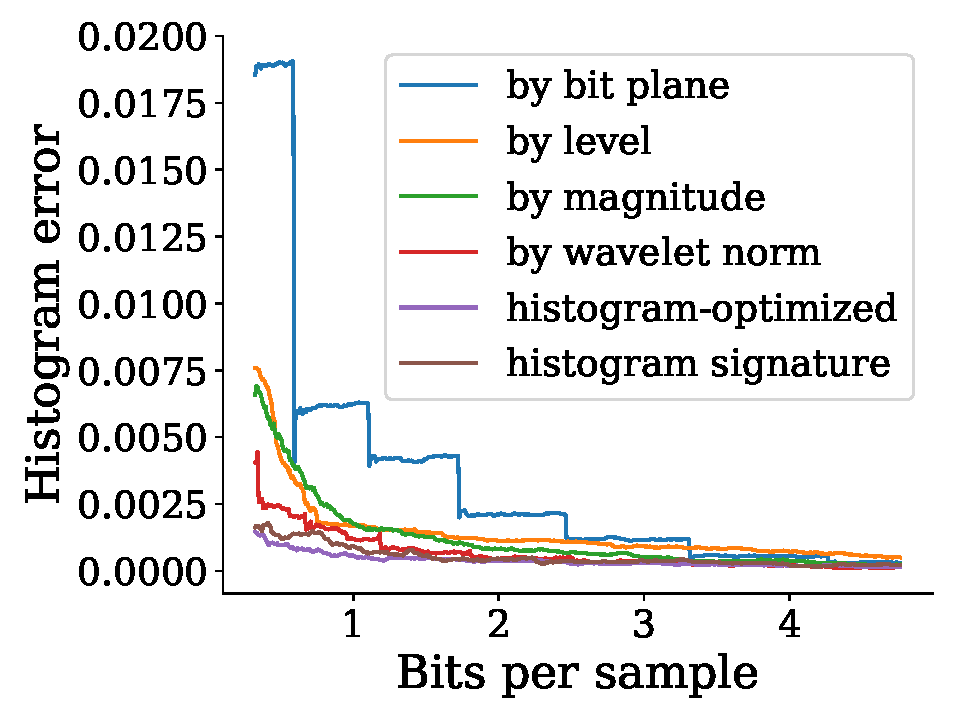
\includegraphics[width=0.24\linewidth]{histogram/histogram-optimized-foam}}
	
	\caption{Comparison of histogram errors among streams. Plots are truncated to highlight
	differences without hiding important trends. In general, in terms of error, $\shop \approx \shsg
	\approx \swav < \slvl, \sbit, \smag$. The erratic behavior at the beginning for \emph{kingsnake}
	is likely due to the data being too noisy. The especially poor performances of \sbit for
	\emph{boiler} and \emph{foam} are due to the ``shifting'' effect explain in~\Cref{sec:gradient}.
	Crossover points between \sbit and \slvl are explained in~\Cref{fig:histogram-explain}}.
	\label{fig:histogram-stream-comparison}
\vspace{1em}

	\centering
	\subcaptionbox{\emph{by level} (\slvl)}{
	{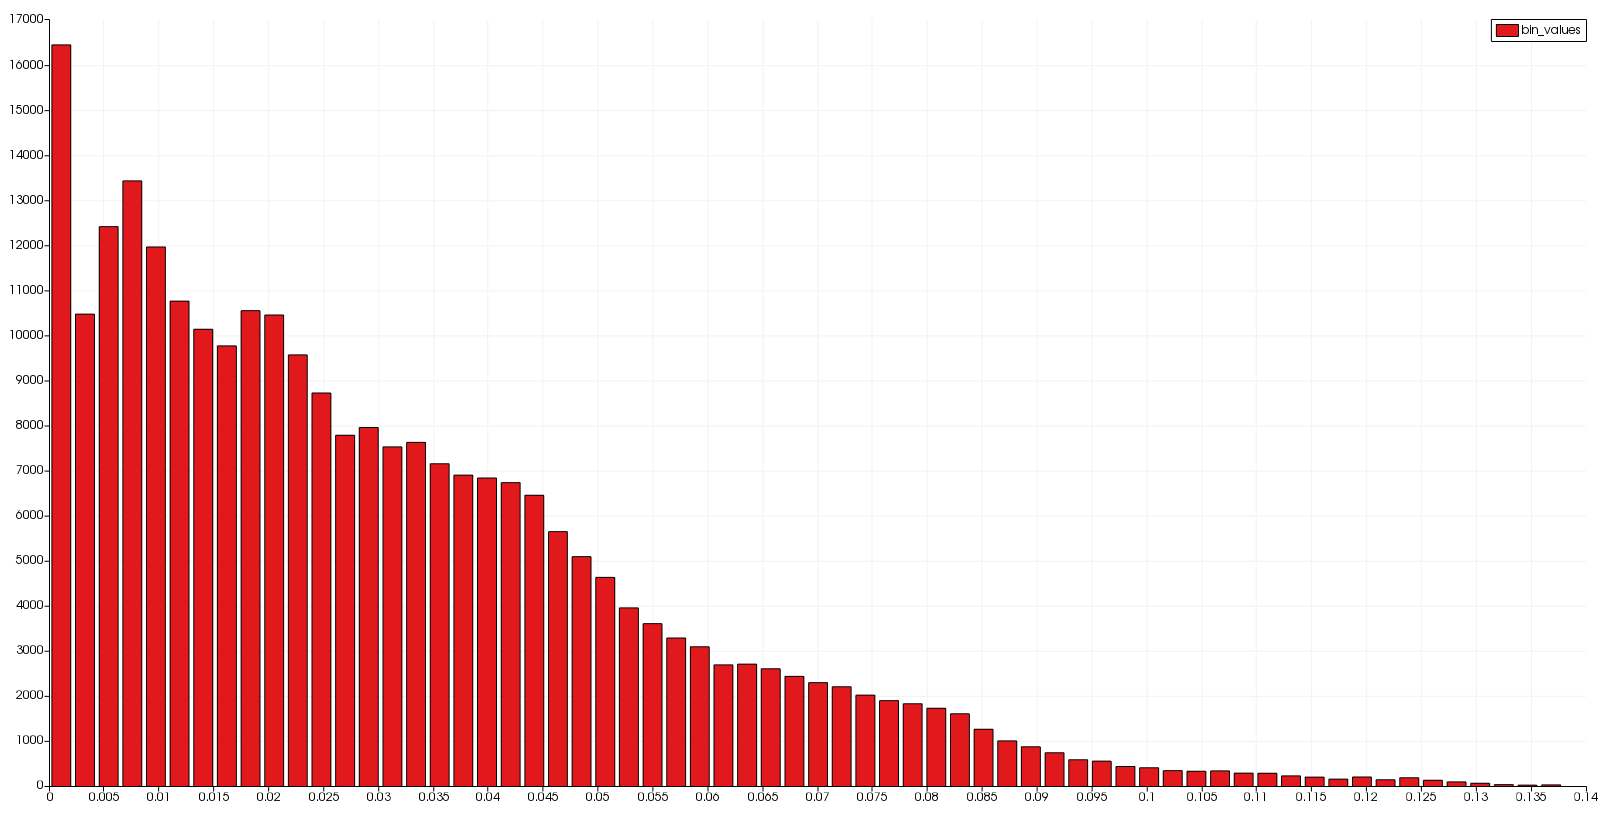
\includegraphics[width=0.155\linewidth]{histogram/histogram-boiler-level.png}}}
	\subcaptionbox{\emph{by bit plane} (\sbit)}{
	{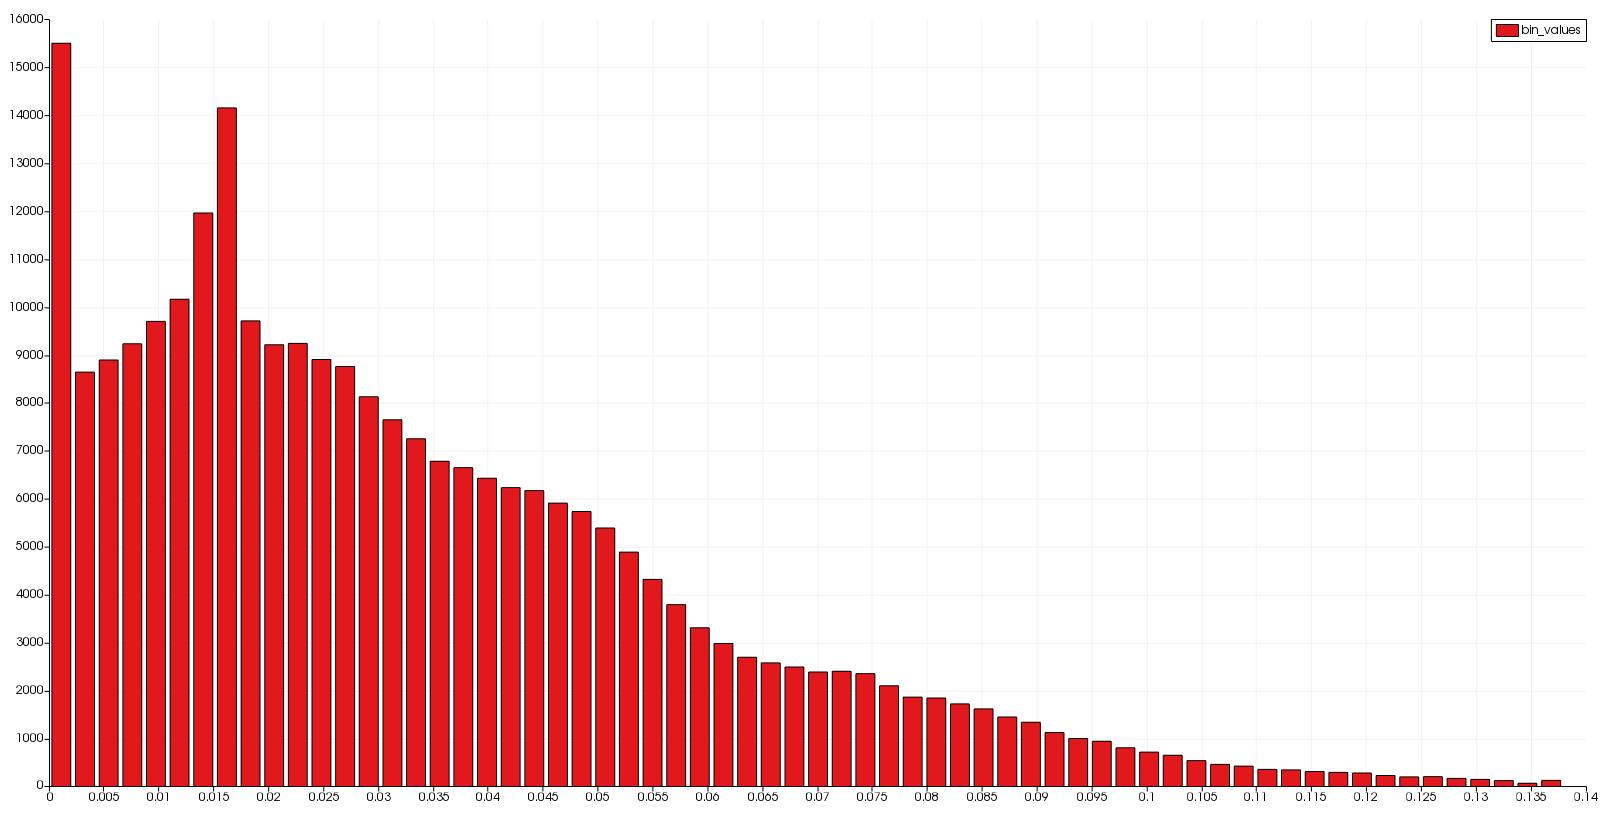
\includegraphics[width=0.155\linewidth]{histogram/histogram-boiler-bit-plane.png}}}
	\subcaptionbox{\emph{by magnitude} (\smag)}{
	{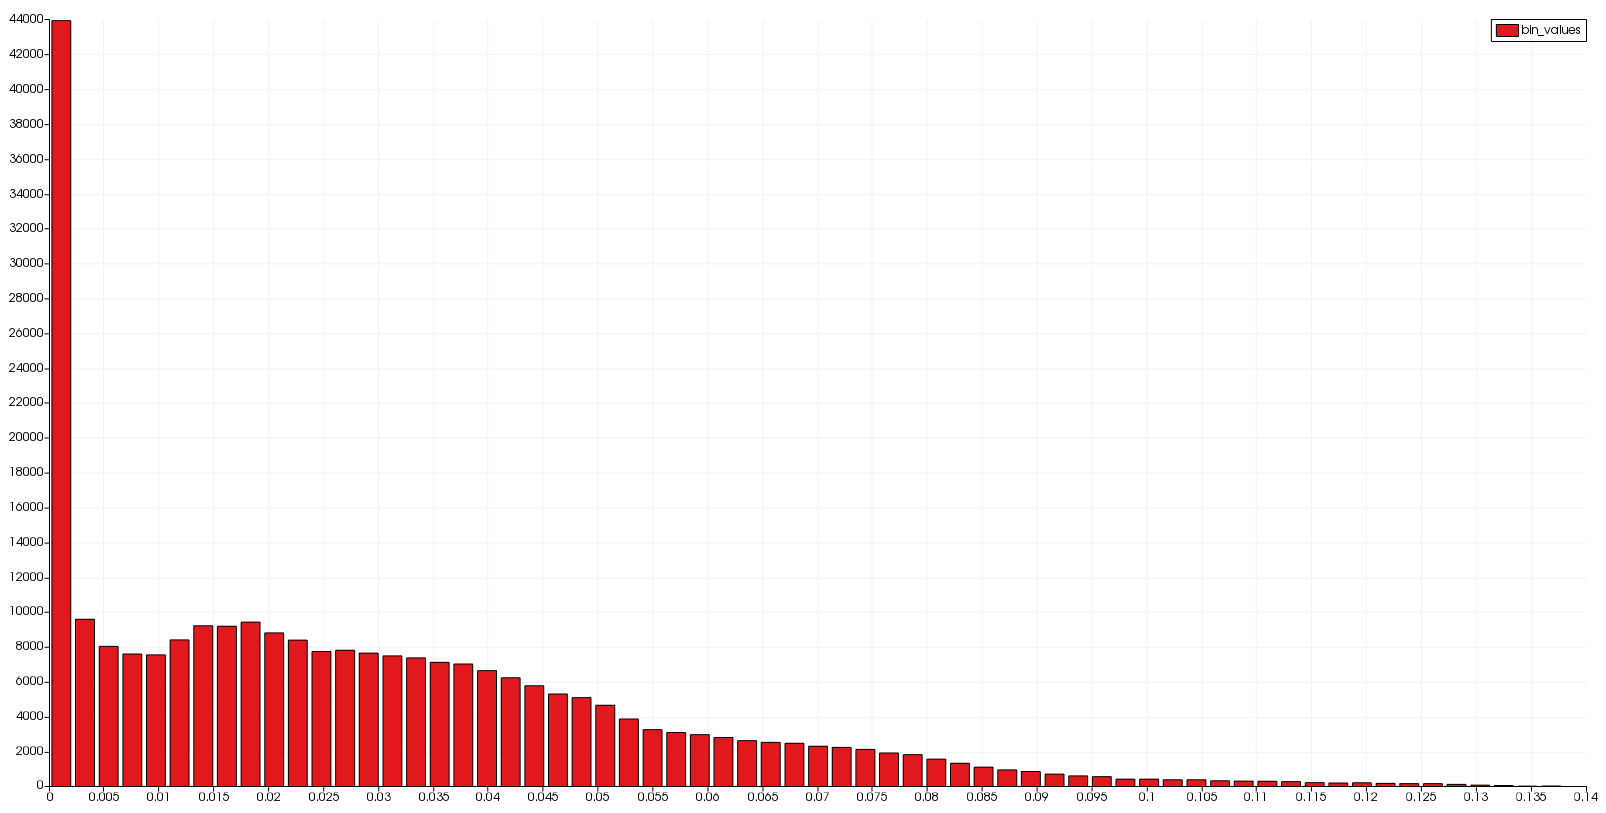
\includegraphics[width=0.155\linewidth]{histogram/histogram-boiler-magnitude.png}}}
	\subcaptionbox{\emph{by wavelet norm} (\swav)}{
	{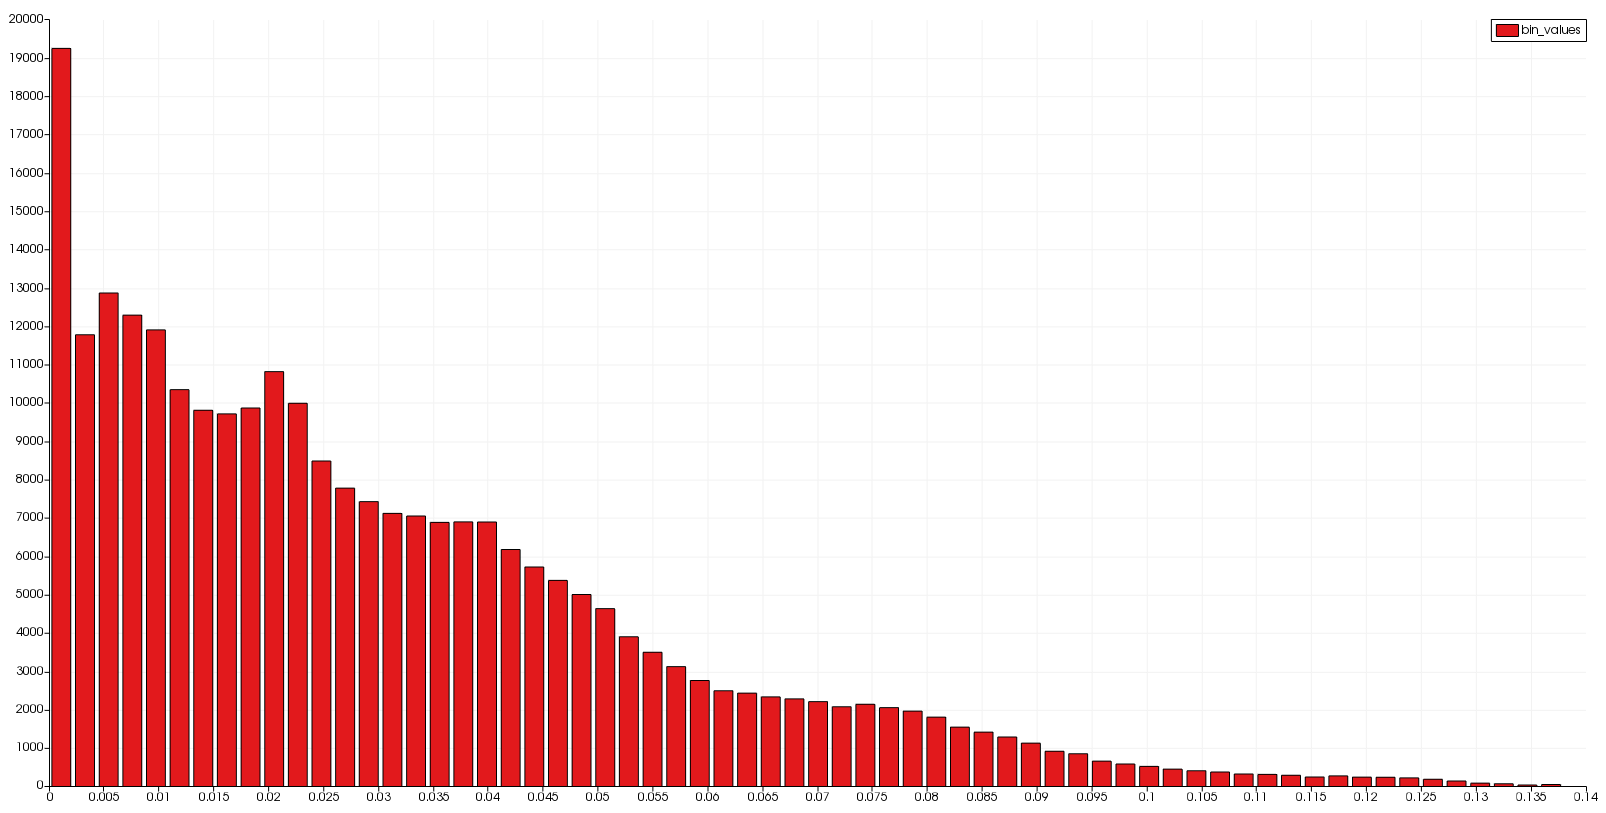
\includegraphics[width=0.155\linewidth]{histogram/histogram-boiler-wavelet-norm.png}}}
	\subcaptionbox{\emph{by signature} (\shsg)}{
	{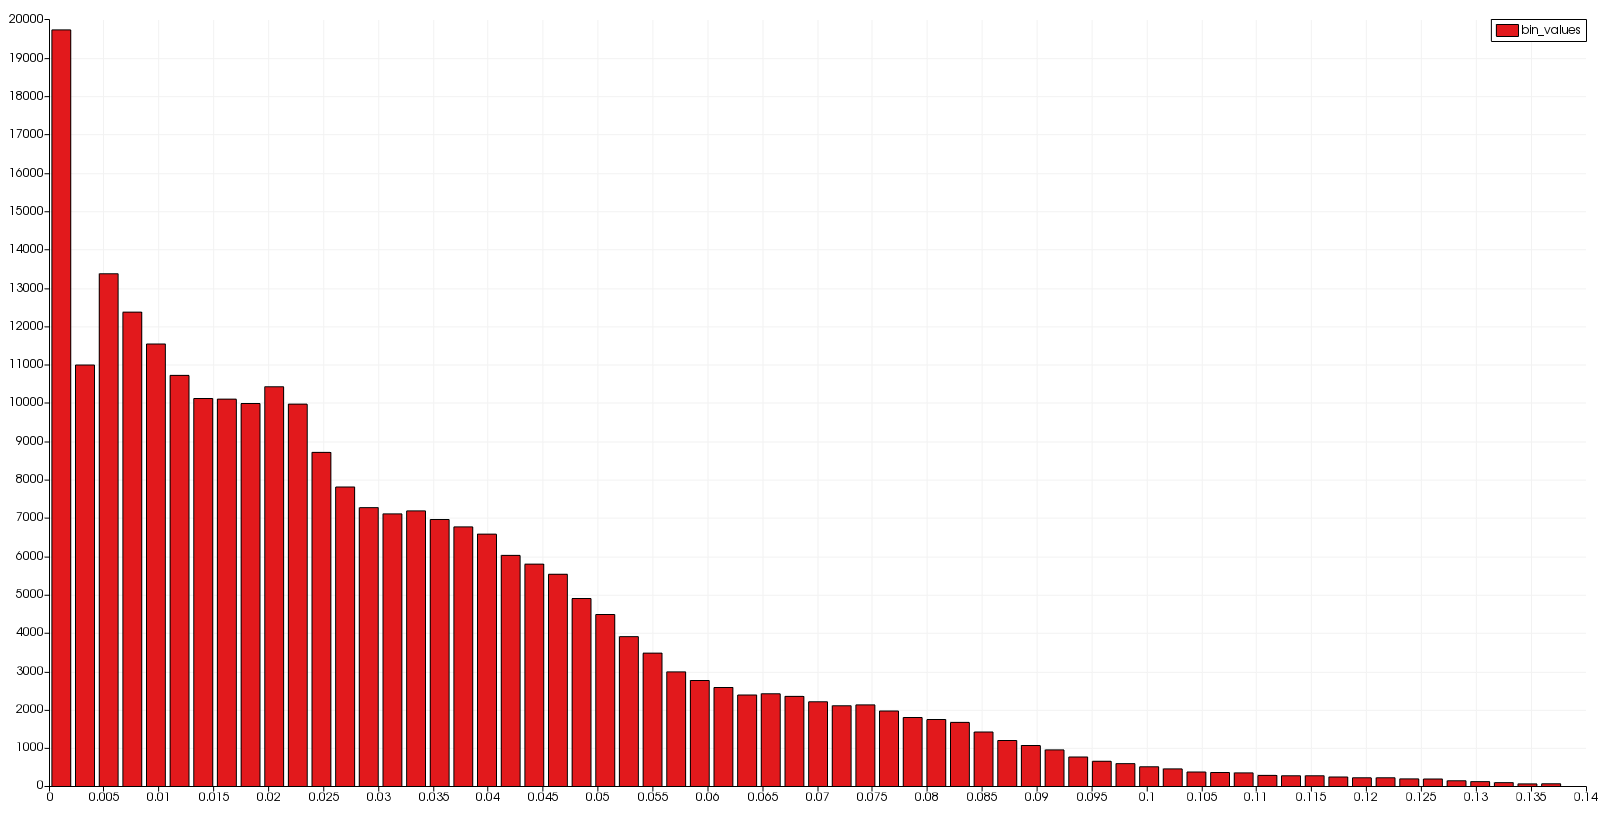
\includegraphics[width=0.155\linewidth]{histogram/histogram-boiler-signature.png}}}
	\subcaptionbox{\emph{reference}}{
	{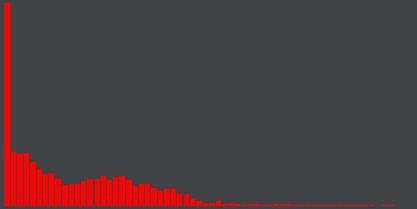
\includegraphics[width=0.155\linewidth]{histogram/histogram-boiler-groundtruth.png}}}
	\caption{Histograms of the \emph{boiler} data set, reconstructed at 0.13 bps. \slvl, \swav, and
	\shsg produce histograms that share a shape similar to the reference histogram, with most of the
	peaks and valleys preserved. In contrast, \sbit produces a spurious peak not found in the
	reference. Finally, \smag's histogram has a widely skewed distribution where too many values fall
	into the first bin.}
	\label{fig:histograms-boiler}
\end{figure*}

\begin{figure*}[t]
\centering
\subcaptionbox{\em pressure, isovalue=0.2}
{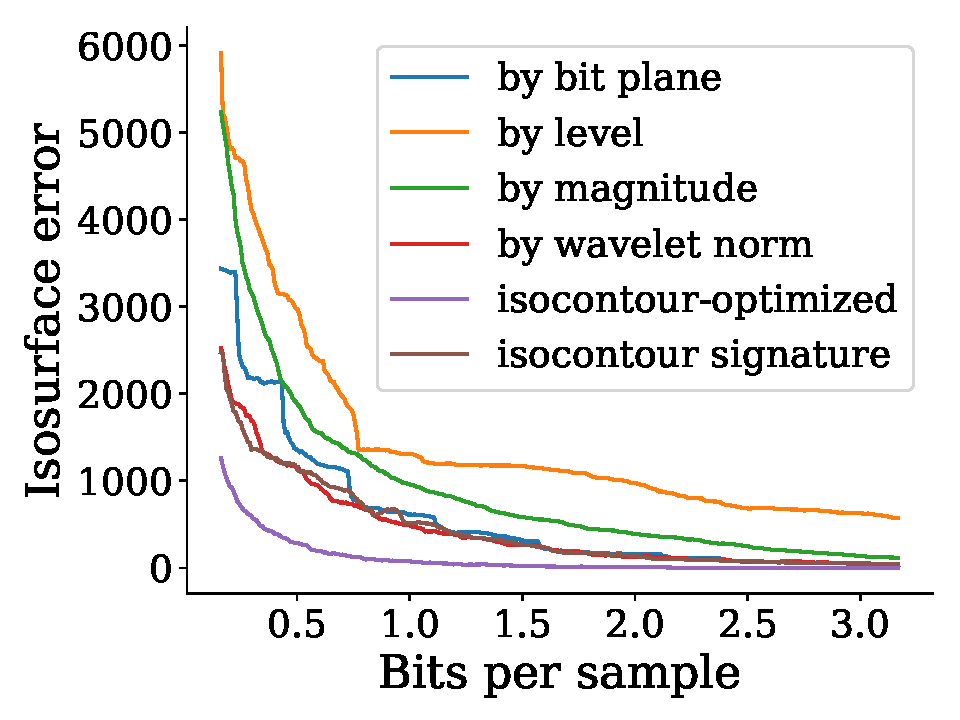
\includegraphics[width=0.24\linewidth]{isocontour/isocontour-optimized-pressure}}
\subcaptionbox{\em kingsnake, isovalue=106}
{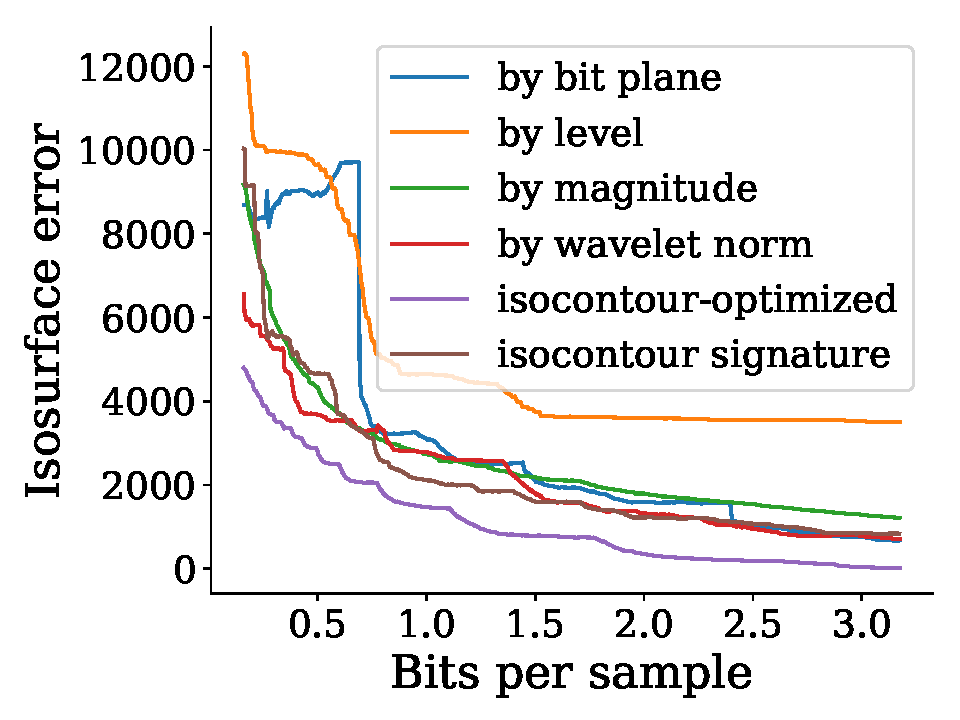
\includegraphics[width=0.24\linewidth]{isocontour/isocontour-optimized-kingsnake}}
\subcaptionbox{\em plasma, isovalue=2}
{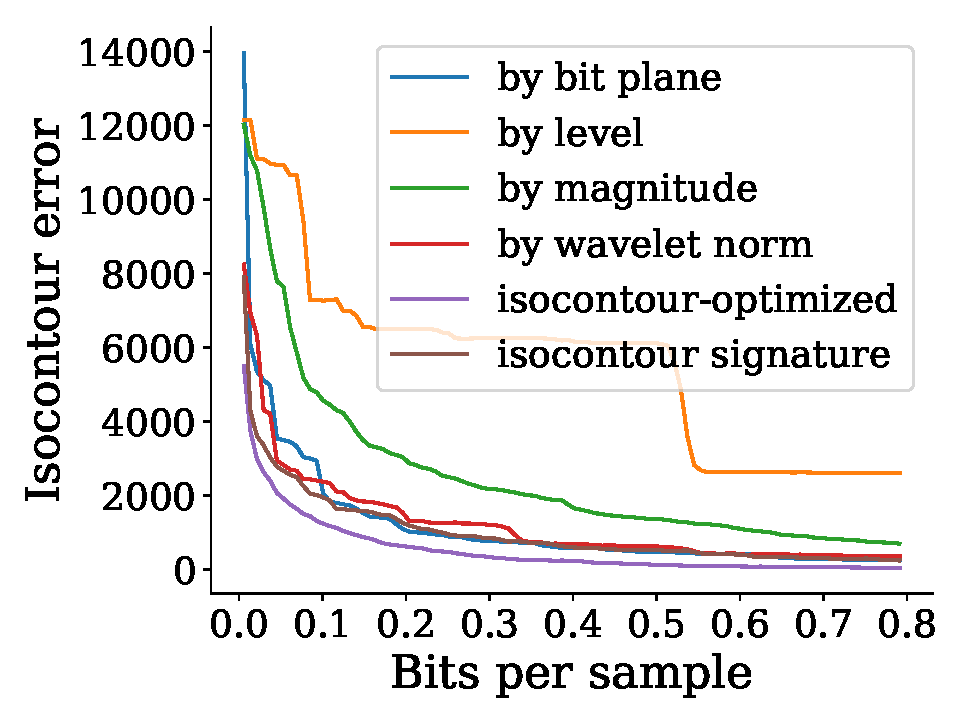
\includegraphics[width=0.24\linewidth]{isocontour/isocontour-optimized-plasma}}
\subcaptionbox{\em turbulence, isovalue=2}
{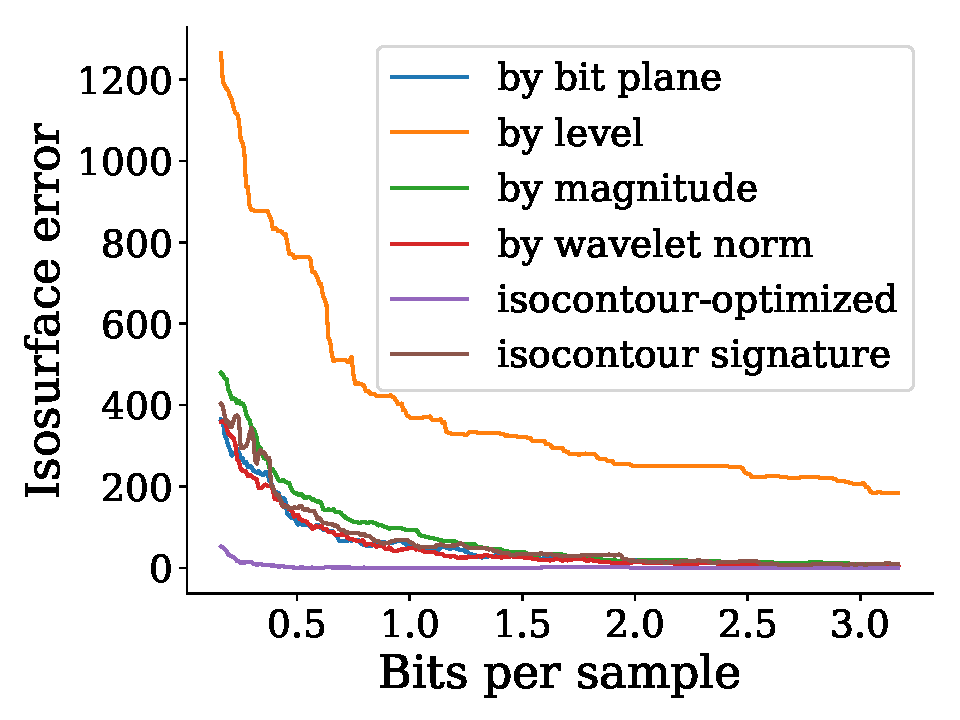
\includegraphics[width=0.24\linewidth]{isocontour/isocontour-optimized-turbulence}}
\caption{Comparison of isosurface errors among streams. Plots are truncated to highlight differences
without hiding important trends. In all cases, \slvl performs significantly worse than the rest.
\swav outperforms \sbit for \emph{pressure} and \emph{kingsnake}, but not for \emph{plasma} and \emph{turbulence}.}\label{fig:isocontour-plots}
\vspace{1em}

\centering
\subcaptionbox{\emph{by level} ($s_{lvl}$)}
{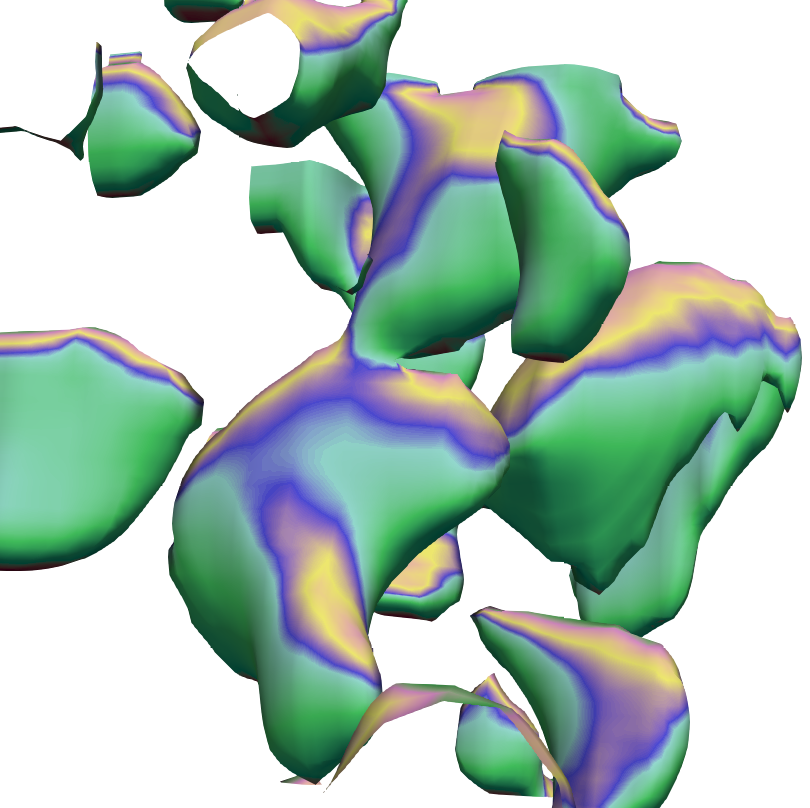
\includegraphics[width=0.16\linewidth]{isocontour/isocontour-level}}
\subcaptionbox{\emph{by bit plane} ($s_{bit}$)}
{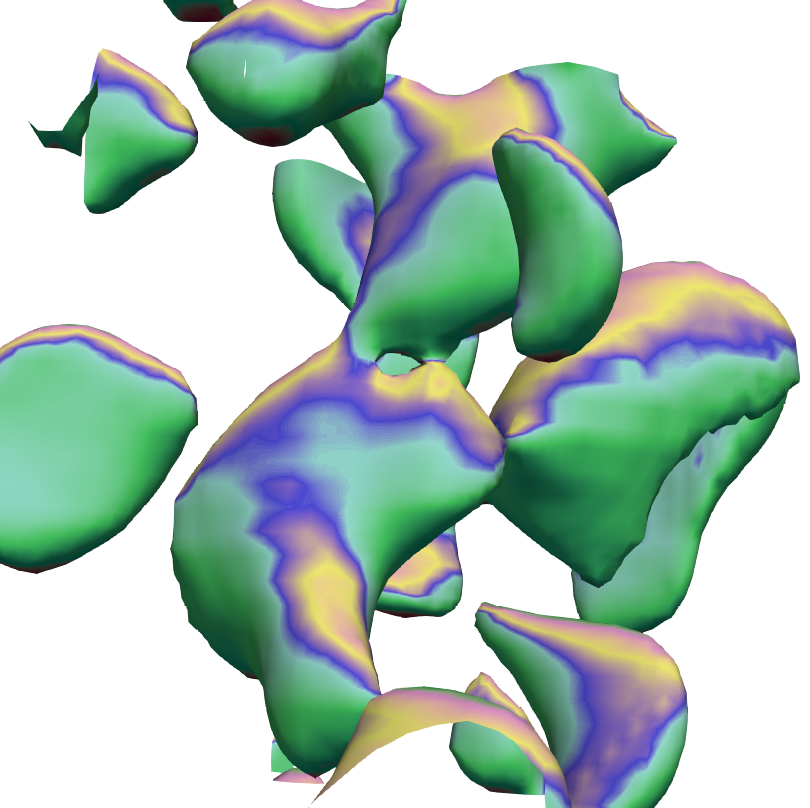
\includegraphics[width=0.16\linewidth]{isocontour/isocontour-bit-plane}}
\subcaptionbox{\emph{by wavelet norm} ($s_{wav}$)}
{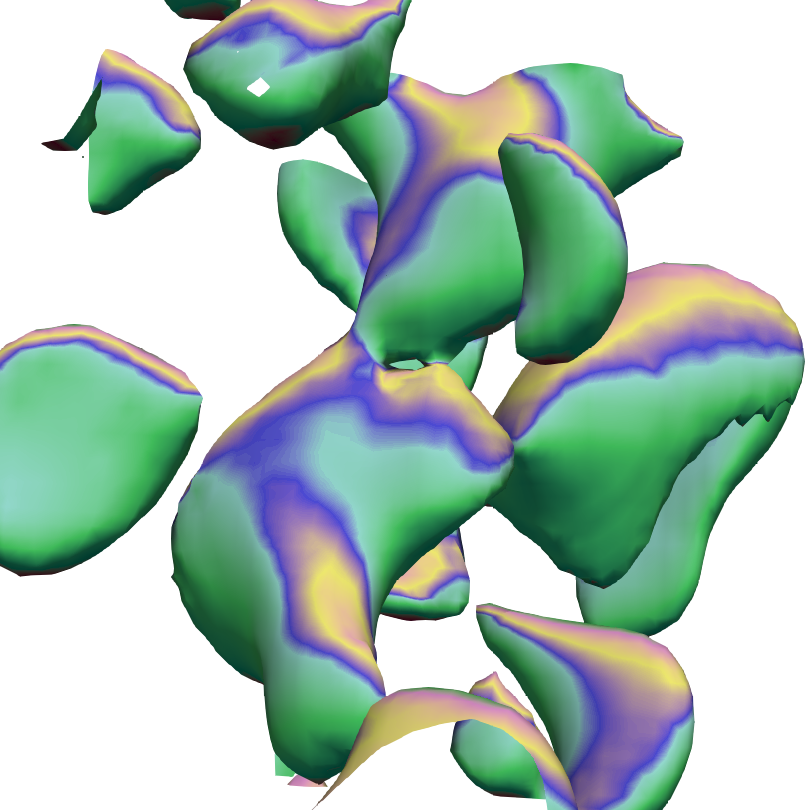
\includegraphics[width=0.16\linewidth]{isocontour/isocontour-wavelet-norm}}
\subcaptionbox{\emph{by magnitude} ($s_{mag}$)}
{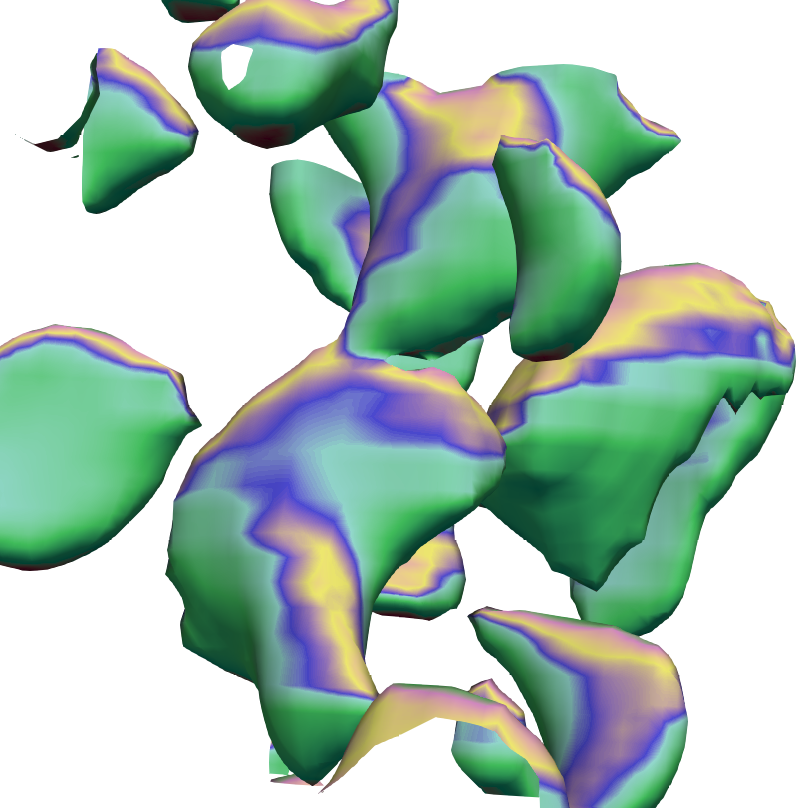
\includegraphics[width=0.16\linewidth]{isocontour/isocontour-magnitude}}
\subcaptionbox{\emph{by signature} ($s_{iso-sig}$)}
{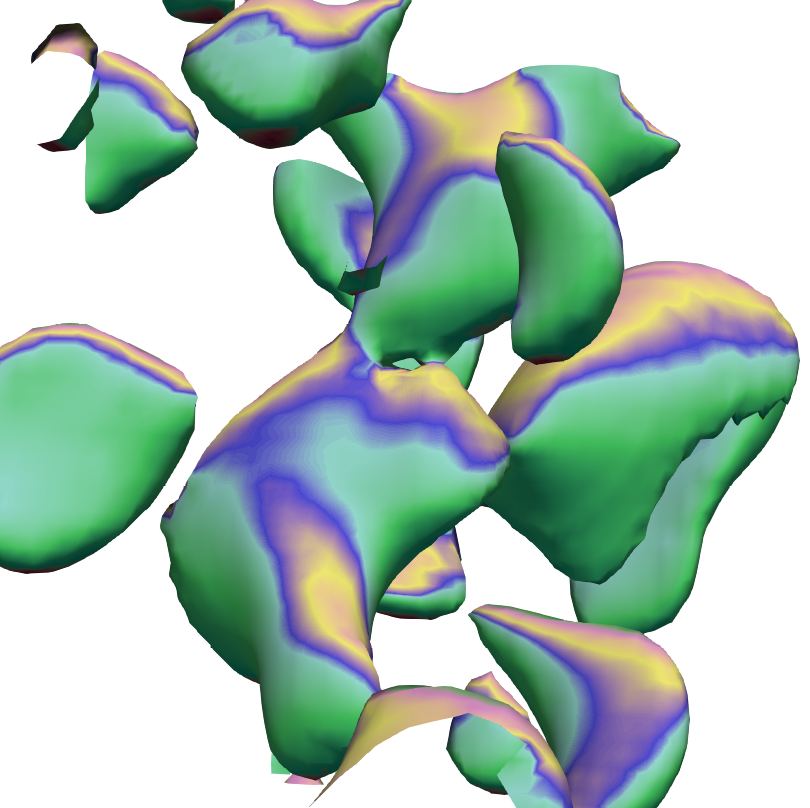
\includegraphics[width=0.16\linewidth]{isocontour/isocontour-signature}}
\subcaptionbox{\emph{ground truth}}
{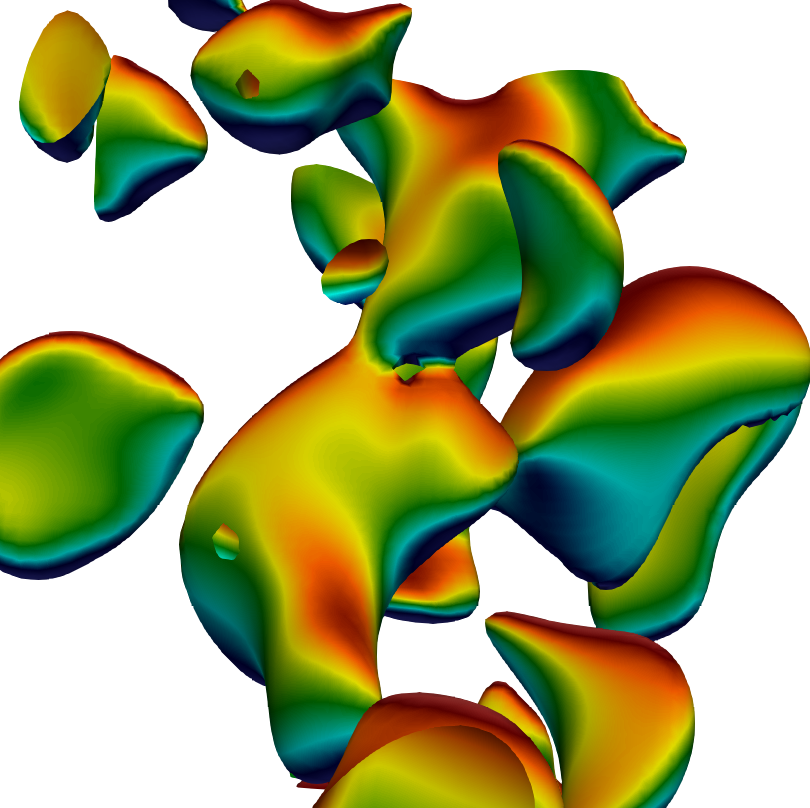
\includegraphics[width=0.16\linewidth]{isocontour/isocontour-groundtruth}}
\caption{Rendering of isosurfaces at isovalue of 0.2, at 0.7 bps, for the \emph{pressure} data set.
The surfaces are colored by the $x$-component of the normal vector at each point. \swav and
\sisg produce surfaces that are closest to the reference, followed by \sbit, \smag, and \slvl.}
\label{fig:isocontour-surfaces-pressure}
\end{figure*}

\begin{figure}[h]
	\centering
	\subcaptionbox{with leading zero packets}
	{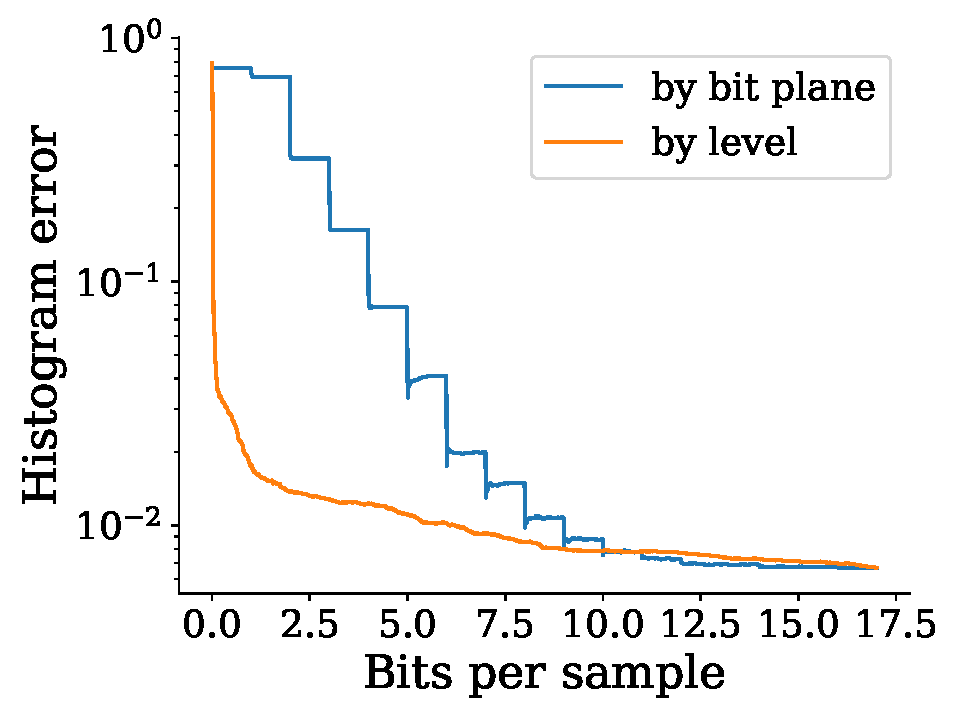
\includegraphics[width=0.48\linewidth]{histogram/histogram-explain-boiler-wlz}}
	\subcaptionbox{without leading zero packets}
	{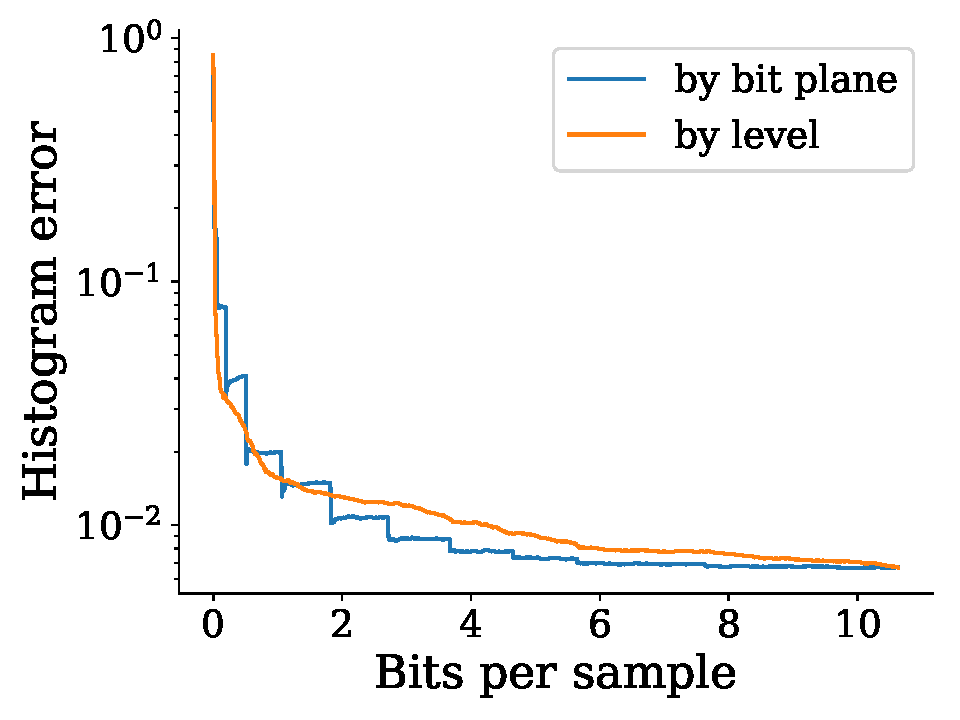
\includegraphics[width=0.48\linewidth]{histogram/histogram-explain-boiler}}
	\caption{Comparison of histogram error curves produced by \sbit and \slvl, for \emph{boiler}, with
	and without leading zero bits. The vertical axis is in log scale. The error for \sbit reduces in a
	stair-step fashion, in which each step corresponds to a new bit plane streamed. \sbit benefits
	significantly more from the removal of leading zero bits (from (a) to (b), the blue curve shifts
	more to the left).}
	\label{fig:histogram-explain}
\end{figure}
